% Provenance (never printed): see sources/outline_sources.md (Year 2: the vanished ocean;
% ophiolites; nappes; high-pressure rocks; foreland basins; reconstructing the history from
% maps, sections and geophysics). Units, ages and architecture after Schmid et al. (2004);
% Monte Cervino sheet notes (ISPRA 2016); Penrose definition as quoted by Coleman (1984);
% Zermatt-Saas ages Rubatto et al. (1998), Halama et al. (2020); Chenaillet Corno et al.
% (2023); Moho picks Michailos et al. (2023, Zenodo, CC BY 4.0); gravity Zahorec et al.
% (2021); Jura Lanza et al. (2022), Schori et al. (2015); shortening Rosenberg et al.
% (2021); Glarus thrust Herwegh et al. (2008); Molasse Krenmayr (1999), Garefalakis and
% Schlunegger (2018), Sinclair (1997); present uplift Champagnac et al. (2009). Figure data
% in figdata/bachelor-2/alps.py; exercise and problem values in the Book 4 scratch
% calculator calc/ch13.py.
\chapter{Anatomy of a Mountain Belt: The Alps}\label{ch:b2:alpine-orogen}

The summit of the Matterhorn is made of gneiss and gabbro that once belonged to the margin
of Apulia, the continent that lay on Africa's side of a vanished ocean. The slopes below
it are that ocean's floor, serpentinite, gabbro and pillow basalt turned to eclogite, and
beneath that, in the neighbouring Monte Rosa, lies the edge of Europe. Climbing through the
pile, one crosses from one continent, through an ocean, to the other. This chapter reads the Alps as such a pile: where its pieces came from, how they were
stacked, how much ground the stacking ate, and what the geophysics sees underneath.
% ledger: ispra16:cervino, schmid04:apulia, schmid04:alpine-tethys

\begin{recall}
\textbf{From the high-school volume}: continental collision, the suture, the shortening of a
layer (the fraction of its length lost), reverse faults and thrusts. \textbf{From the Year 1
volume}: geological maps and cross-sections; normal, reverse and thrust faults, folds and
vergence; passive margins; the oceanic crust, pillow lava and the sheeted \omterm{def:b2:magma-emplacement:bodies}{dyke} complex;
active margins and the accretionary prism; isostasy, Airy's root and the Bouguer anomaly;
the \omterm{def:b2:alpine-orogen:foreland}{foreland basin} named among sedimentary basins. \textbf{From
\cref{ch:b2:metamorphic-facies}}: the blueschist and eclogite facies. \textbf{From
\cref{ch:b2:pt-paths}}: \omterm{def:b2:pt-paths:ptt}{P--T--t paths}, \omterm{def:b2:pt-paths:exhumation}{exhumation rates} and \omterm{def:b2:pt-paths:uhp}{ultrahigh-pressure
metamorphism}.
\end{recall}

\begin{definition}[Orogen]\label{def:b2:alpine-orogen:orogen}
An \emph{orogen}\index{orogen} is a belt of the lithosphere shortened and thickened by the
convergence of two plates, together with the rocks deformed and metamorphosed in it; the
mountain range is its surface expression, the thickened crust beneath is its root.
\end{definition}

\section{A vanished ocean}\label{sec:b2:alpine-orogen:tethys}

The Alps record the closure of oceans while the African and European plates converged.
The main one is the \emph{Alpine Tethys}, made of two branches. Its southern branch, the
Piemont--Liguria ocean, began to drift apart in the Middle Jurassic, as the Central Atlantic
opened: the Alpine Tethys belongs kinematically to the opening of the Atlantic, unlike the
Tethyan oceans further east. Radiolarites, siliceous oozes of the deep sea turned to rock,
and aptychus limestones followed the onset of spreading, and they still identify its
remnants. A narrow northern branch, the Valais ocean, probably opened in the earliest
Cretaceous. Between the two lay a sliver of continent, the Briançonnais ribbon, which thins
out eastwards and is absent from the eastern Alps.
% ledger: schmid04:alpine-tethys

To the north the ocean was bordered by Europe's passive margin, the subject of the rift and
margin chapter of the Year 1 volume. To the south lay \emph{Apulia}: all the continental
ground south of the Alpine Tethys and north of the younger Neotethys, including the foreland
that now lies south of the Alps. The Matterhorn's summit is a piece of it.
% ledger: schmid04:apulia
The map below locates the belt and the places of this chapter.

\begin{omfigure}
\centering
% ledger: data:b4-etopo-alps, schmid04:windows, schmid04:foreland, ispra16:cervino
\begin{tikzpicture}
\begin{axis}[width=0.96\linewidth, height=0.74\linewidth, xmin=5, xmax=14, ymin=43.5,
  ymax=48.5, xlabel={longitude (\unit{\degree} E)}, ylabel={latitude (\unit{\degree} N)},
  tick label style={font=\scriptsize}, label style={font=\small}, clip=true,
  xtick={5,6,...,14}, ytick={44,45,...,48}]
\addplot[omThm!35, line width=0.3pt] table[x=lon, y=lat] {figdata/out/bachelor-2-alps-c1000.dat};
\addplot[omThm!90!black, line width=0.45pt] table[x=lon, y=lat] {figdata/out/bachelor-2-alps-c2000.dat};
\addplot[blue!60!black, line width=0.5pt] table[x=lon, y=lat] {figdata/out/bachelor-2-alps-c0.dat};
\draw[red!70!black, line width=1pt] (axis cs:8,45.3) -- (axis cs:8,48.0);
\node[font=\scriptsize\bfseries, red!70!black, anchor=north west] at (axis cs:8.02,45.32) {A};
\node[font=\scriptsize\bfseries, red!70!black, anchor=south west] at (axis cs:8.02,47.98) {B};
\fill (axis cs:6.865,45.833) circle (1.3pt) node[font=\scriptsize, fill=white, fill opacity=0.85, text opacity=1, inner sep=1pt, anchor=north east] {Mont Blanc};
\fill (axis cs:7.659,45.976) circle (1.3pt) node[font=\scriptsize, fill=white, fill opacity=0.85, text opacity=1, inner sep=1pt, anchor=south east] {Matterhorn};
\node[font=\scriptsize\itshape, rotate=40] at (axis cs:6.35,46.85) {Jura};
\node[font=\scriptsize\itshape] at (axis cs:9.35,47.65) {Molasse basin};
\node[font=\scriptsize\itshape] at (axis cs:10.0,45.05) {Po plain};
\node[font=\scriptsize\itshape, align=center, fill=white, fill opacity=0.8, text opacity=1, inner sep=1pt] at (axis cs:10.3,46.95) {Engadine\\window};
\node[font=\scriptsize\itshape, align=center, fill=white, fill opacity=0.8, text opacity=1, inner sep=1pt] at (axis cs:12.6,47.25) {Tauern\\window};
\node[font=\scriptsize\itshape] at (axis cs:8.6,43.85) {Ligurian Sea};
\end{axis}
\end{tikzpicture}
\par\smallskip{\small The Alps from the ETOPO1 relief model, every node \qty{0.05}{\degree}
apart: contours at \qty{1000}{m} (light) and \qty{2000}{m} (dark) and the coastline. The
highest node of this grid is \qty{3914}{m}, near Mont Blanc; the summits stand higher,
because a grid node samples a cell, not a peak. The line A--B along \qty{8}{\degree} E is
the profile drawn in the last section of the chapter. Feature names placed by hand at their
approximate positions.}
\end{omfigure}

How can an ocean that has gone be known? By pieces of its floor that escaped
subduction and were caught in the mountain belt.

\begin{definition}[Ophiolite; Penrose ophiolite sequence]\label{def:b2:alpine-orogen:ophiolite}
An \emph{ophiolite}\index{ophiolite} is a distinctive assemblage of mafic to ultramafic
rocks, a piece of oceanic lithosphere now found on land. The \emph{Penrose ophiolite
sequence}\index{Penrose ophiolite sequence} is the complete assemblage defined by a
conference of geologists in 1972; from bottom to top:
\begin{enumerate}
\item an ultramafic complex of \omterm{def:b2:mantle-melting:peridotites}{harzburgite}, \omterm{def:b2:mantle-melting:peridotites}{lherzolite} and \omterm{def:b2:mantle-melting:peridotites}{dunite}, usually with a
deformation fabric acquired in the solid state;
\item a gabbroic complex, ordinarily with cumulus textures;
\item a mafic sheeted \omterm{def:b2:magma-emplacement:bodies}{dyke} complex;
\item a mafic volcanic complex, commonly pillowed.
\end{enumerate}
\end{definition}
% ledger: coleman84:penrose

The Penrose definition was a consensus, criticised from the start, and still generally
accepted. Its sequence is the layering of the oceanic crust and upper mantle met in the Year 1
volume: pillow lavas over sheeted \omterm{def:b2:magma-emplacement:bodies}{dykes} over gabbro over the mantle. \omterm{def:b2:alpine-orogen:ophiolite}{Ophiolites}, however, are not
average ocean floor. Most abyssal crust, the crust of the wide oceans, is consumed by
subduction; Coleman argued that the \omterm{def:b2:alpine-orogen:ophiolite}{ophiolites} of the Alpine and Cordilleran belts formed
mainly at the spreading centres of small ocean basins or between island arcs, and that the
Tethyan ones formed where continental crust thinned along passive margins until a small
ocean opened.
% ledger: coleman84:penrose, coleman84:settings

The Alpine \omterm{def:b2:alpine-orogen:ophiolite}{ophiolites} fit that picture. The units derived from the Piemont--Liguria ocean
are relics of oceanic lithosphere and of mantle that had been brought up from beneath the
thinned continent, the sub-continental mantle, and exposed on the sea floor. At the
Chenaillet, in the Western Alps, the best preserved of them shows exposed
mantle, gabbros and a famous sequence of pillow basalts, with no sedimentary cover.
The photograph below shows them.
% ledger: schmid04:units, corno23:chenaillet

\begin{omfigure}
\centering
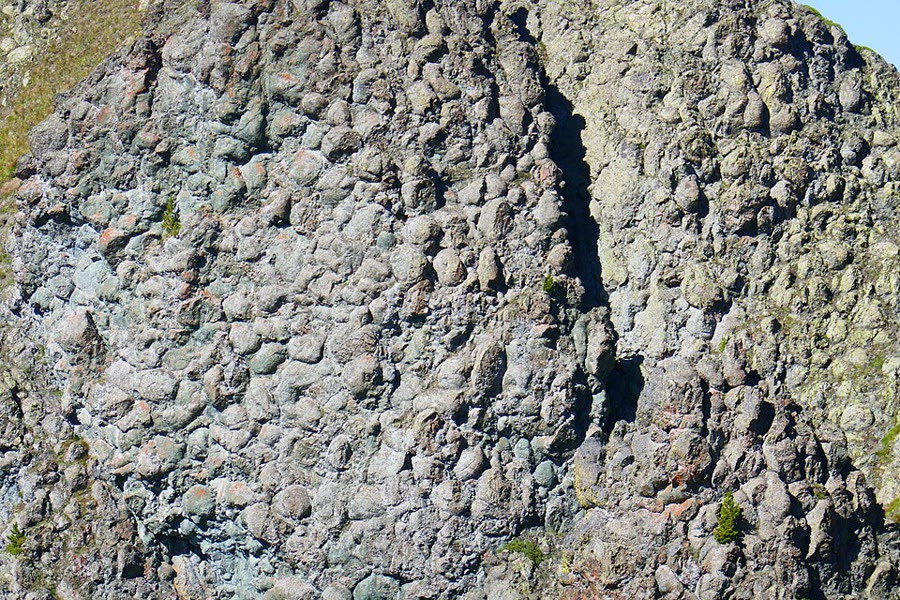
\includegraphics[width=0.66\linewidth]{images/book4/b2-13-pillow-lava.jpg}
\par\smallskip{\small Pillow lavas of the Chenaillet \omterm{def:b2:alpine-orogen:ophiolite}{ophiolite}, Western Alps: each rounded
cushion is a lobe of basalt that erupted and chilled on the floor of the Piemont--Liguria
ocean. Photograph Lionel Duchoiselle, CC BY-SA 3.0.}
\end{omfigure}

The ocean floor can be dated where its gabbros crystallised. Zircons from two metagabbros of
the Zermatt--Saas \omterm{def:b2:alpine-orogen:ophiolite}{ophiolite}, below the Matterhorn, give $164.0 \pm \qty{2.7}{Ma}$ and $163.5
\pm \qty{1.8}{Ma}$, and the manganese-rich sediments laid on the basalts are at most $161
\pm \qty{11}{Ma}$ old: the floor of the Piemont--Liguria ocean was forming in the Jurassic,
about \qty{164}{Myr} ago.
% ledger: rubatto98:zsf

\section{Subducting an ocean, then a continent}\label{sec:b2:alpine-orogen:subduction}

An ocean closes by subduction. Some of its floor, though, ends up on top of a continent
rather than beneath it, and some continents follow the ocean down.

\begin{definition}[Obduction; continental subduction]\label{def:b2:alpine-orogen:obduction}
\emph{Obduction}\index{obduction} is the emplacement of a slab of oceanic lithosphere onto
a continental margin, the \omterm{def:b2:alpine-orogen:ophiolite}{ophiolite} riding over the continent. \emph{Continental
subduction}\index{continental subduction} is the descent of continental lithosphere, pulled
by the oceanic slab attached to it, into a subduction zone after the ocean in front of it
has been consumed.
\end{definition}

\omterm{def:b2:alpine-orogen:obduction}{Obduction} happened in the Dinarides, south-east of the Alps: \omterm{def:b2:alpine-orogen:ophiolite}{ophiolites} of the Jurassic
Vardar ocean, themselves of Middle Jurassic age, were thrust in the Late Jurassic onto an
accretionary wedge and onto the margin of Apulia. It was long thought to have placed the
Chenaillet \omterm{def:b2:alpine-orogen:ophiolite}{ophiolite} as well, because its rocks show only very low-grade Alpine
\omterm{def:b2:metamorphic-facies:metamorphism}{metamorphism}. A recent study found relics of lawsonite and omphacite in its gabbro and
albitite, which put its Alpine peak at 10 to \qty{11}{kbar} and 340 to
\qty{360}{\celsius}: the weight of a \omterm{def:b2:alpine-orogen:nappes}{nappe} pile some 35 to \qty{40}{km} thick. The authors
conclude that the Chenaillet was subducted, not obducted, a reminder that the reading of
an \omterm{def:b2:alpine-orogen:ophiolite}{ophiolite} rests on its metamorphic history as much as on its rocks.
% ledger: schmid04:obduction, corno23:chenaillet

\subsection*{The ocean goes down}

In the Cretaceous the southern, Apulian margin of the Piemont--Liguria ocean became an
active margin: its trench filled with shales and sandstones, now the calcareous schists
called Bündnerschiefer or schistes lustrés. The eastern Alps also record an earlier
collision, the closure of a gulf of another ocean, the Meliata, into Apulia, with a
high-pressure peak at around \qty{100}{Ma}: the Alps are the product of two orogenies, a
Cretaceous one and a Tertiary one.
% ledger: schmid04:two-orogenies

The Zermatt--Saas \omterm{def:b2:alpine-orogen:ophiolite}{ophiolite} went down to the eclogite facies of
\cref{ch:b2:metamorphic-facies}: its eclogites reached 550 to \qty{600}{\celsius} and 2.5 to
\qty{3.0}{GPa}, and peak pressure was reached between 48 and \qty{44}{Ma}. One slice of it,
at Lago di Cignana, holds coesite and microscopic diamonds in rocks that began as basalts
and ocean-floor sediments; it reached about \qty{615}{\celsius} and \qty{2.8}{GPa}, and its
zircons date that deepest point at $44.1 \pm \qty{0.7}{Ma}$. Ocean floor born
\qty{164}{Myr} ago was subducted, at the age of 120 million years, to depths of
\qty{90}{km} or more, then came back.
% ledger: halama20:cignana, rubatto98:zsf

\subsection*{The continent follows}

When the ocean had gone, Europe's margin was dragged after it. The coesite-bearing
quartzites of the Dora Maira massif, met in \cref{ch:b2:pt-paths}, are continental crust
from the European side of the ocean that reached more than \qty{90}{km}, about
\qty{35}{Myr} ago, and came back at the speed of plates. Dating the high-pressure rocks
across the belt gives an order: the Apulian margin itself (the Sesia zone) in the Late
Cretaceous, the \omterm{def:b2:alpine-orogen:ophiolite}{ophiolites} of the Piemont--Liguria ocean at about \qty{44}{Ma}, the
European continental crust in the late Eocene. Rubatto and colleagues read it as three episodes of subduction stepping in time from
south-east to north-west, towards Europe.
% ledger: chopin84:coesite, rh01:exhumation, rubatto98:zsf, ispra16:cervino

Collision followed: the Valais ocean, the last oceanic strip, closed during the middle to
late Eocene, and from then on continental crust was stacked on continental crust.
The figure below sums up the sequence.
% ledger: schmid04:alpine-tethys

\begin{omfigure}
\centering
\begin{tikzpicture}[x=0.95cm, y=0.78cm, font=\scriptsize]
% (a) rifting and spreading
\begin{scope}[yshift=0cm]
\node[anchor=west, font=\scriptsize\bfseries] at (-0.2,0.75) {(a) Jurassic: the ocean opens};
\fill[gray!25] (0,0) -- (3.2,0) -- (3.8,-0.6) -- (0,-0.6) -- cycle;
\fill[gray!25] (6.2,0) -- (10,0) -- (10,-0.6) -- (5.6,-0.6) -- cycle;
\fill[omThm!35] (3.2,0) -- (6.2,0) -- (5.6,-0.6) -- (3.8,-0.6) -- cycle;
\fill[blue!8] (0,0) rectangle (10,0.4);
\draw[thick] (4.7,0) -- (4.7,-0.6);
\node at (1.6,-0.3) {Europe};
\node at (8,-0.3) {Apulia};
\node[align=center] at (4.7,0.2) {ridge};
\end{scope}
% (b) oceanic subduction
\begin{scope}[yshift=-1.7cm]
\node[anchor=west, font=\scriptsize\bfseries] at (-0.2,0.75) {(b) Cretaceous to Eocene: the ocean is subducted};
\fill[blue!8] (0,0) rectangle (7,0.4);
\fill[gray!25] (0,0) -- (3.0,0) -- (3.6,-0.6) -- (0,-0.6) -- cycle;
\fill[omThm!35] (3.0,0) -- (6.3,0) -- (6.0,-0.5) -- (5.6,-0.95) -- (3.6,-0.6) -- cycle;
\fill[gray!25] (6.3,0) -- (6.6,0.3) -- (10,0.3) -- (10,-0.6) -- (6.4,-0.6) -- cycle;
\fill[omThm!35] (5.6,-0.95) -- (6.0,-0.5) -- (7.4,-1.3) -- (7.2,-1.55) -- cycle;
\fill[orange!40] (6.0,0) -- (6.3,0) -- (6.6,0.3) -- (6.35,0.3) -- cycle;
\draw[-{Latex[length=2mm]}] (7.0,-1.0) -- (7.6,-1.38);
\node at (1.6,-0.3) {Europe};
\node at (8.4,-0.15) {Apulia};
\node[anchor=west] at (7.5,-1.1) {eclogite};
\end{scope}
% (c) continental subduction
\begin{scope}[yshift=-3.95cm]
\node[anchor=west, font=\scriptsize\bfseries] at (-0.2,0.75) {(c) Eocene: the European margin follows};
\fill[gray!25] (0,0) -- (5.6,0) -- (6.2,-0.5) -- (7.4,-1.35) -- (7.1,-1.6) -- (5.6,-0.6) -- (0,-0.6) -- cycle;
\fill[omThm!35] (6.2,0.05) -- (6.6,0.3) -- (6.95,0.3) -- (6.4,-0.2) -- cycle;
\fill[gray!25] (6.6,0.3) -- (10,0.3) -- (10,-0.6) -- (6.9,-0.6) -- (6.4,-0.2) -- (6.95,0.3) -- cycle;
\draw[dashed] (6.6,-0.85) circle (0.22);
\draw (6.82,-0.9) -- (7.6,-1.2);
\node[anchor=west] at (7.6,-1.2) {UHP continental crust};
\node at (2.4,-0.3) {Europe};
\node at (8.4,-0.15) {Apulia};
\end{scope}
% (d) collision
\begin{scope}[yshift=-6.65cm]
\node[anchor=west, font=\scriptsize\bfseries] at (-0.2,1.4) {(d) Oligocene to present: collision, nappes, foreland basins};
\fill[yellow!35] (0.6,0) -- (3.4,0) -- (3.4,-0.3) -- cycle;
\fill[gray!25] (0,-0.3) -- (3.4,-0.3) -- (4.2,0.5) -- (5.2,0.75) -- (6.2,0.55) -- (7.0,0.2) -- (10,0.2)
  -- (10,-0.7) -- (6.6,-0.7) -- (5.4,-1.5) -- (4.0,-1.5) -- (3.2,-0.9) -- (0,-0.9) -- cycle;
\draw (3.4,-0.3) -- (4.5,-1.0);
\draw (4.2,0.5) -- (5.6,-0.4);
\draw (5.2,0.75) -- (6.1,0.1);
\fill[omThm!35] (5.05,0.6) -- (5.55,0.68) -- (5.85,0.32) -- (5.4,0.25) -- cycle;
\fill[yellow!35] (7.0,0.2) -- (9.6,0.2) -- (7.0,-0.1) -- cycle;
\node at (1.4,-0.6) {Europe};
\node at (8.6,-0.3) {Apulia};
\node[anchor=south] at (1.9,0.02) {molasse};
\node at (4.7,-1.25) {root};
\node[anchor=south west] at (6.25,0.6) {nappe stack};
\end{scope}
\end{tikzpicture}
\par\smallskip{\small A schematic history of the Alps, not to scale (oceanic lithosphere red,
continental grey, accretionary wedge orange, \omterm{def:b2:alpine-orogen:foreland}{foreland basins} yellow).
(a)~The Piemont--Liguria ocean opens between Europe and Apulia. (b)~Its floor is subducted
beneath Apulia and turned to eclogite. (c)~The European margin is pulled down after it and
metamorphosed at ultrahigh pressure. (d)~Continental crust is stacked into \omterm{def:b2:alpine-orogen:nappes}{nappes} over a
thickened root, with flexural \omterm{def:b2:alpine-orogen:foreland}{foreland basins} on both sides.}
\end{omfigure}
% ledger: schmid04:alpine-tethys, schmid04:two-orogenies, rubatto98:zsf, schmid04:foreland

\section{Nappes, klippen and windows}\label{sec:b2:alpine-orogen:nappes}

The pieces of ocean and continent were not piled up whole. They were scraped off as thin
slices and carried far.

\begin{definition}[Nappe; nappe stack]\label{def:b2:alpine-orogen:nappes}
A \emph{nappe}\index{nappe} is a large sheet of rock, often a few kilometres thick and tens
of kilometres long, carried along a low-angle thrust or in the overturned limb of a large
recumbent fold far from its place of origin; the rocks of a nappe are
\emph{allochthonous}\index{allochthonous (rock unit)}, those that stayed in place
\emph{autochthonous}\index{autochthonous (rock unit)}. A \emph{nappe
stack}\index{nappe stack} is a pile of nappes in which the structurally higher nappes
usually come from farther inside the \omterm{def:b2:alpine-orogen:orogen}{orogen}.
\end{definition}

In the Alps the stacking order is the geography of the vanished ocean turned upside down,
and the units are named by their origin (table below).

\begin{omfigure}
\centering\small
\begin{tabular}{>{\raggedright\arraybackslash}p{0.24\linewidth}|>{\raggedright\arraybackslash}p{0.66\linewidth}}
unit (top to bottom) & origin and rocks \\ \hline
Austroalpine \omterm{def:b2:alpine-orogen:nappes}{nappes} & margin of Apulia north of the Periadriatic Line: basement and cover
slices detached from their lower crust \\
Margna--Sesia \omterm{def:b2:alpine-orogen:nappes}{nappes} (Sesia zone, Dent Blanche) & fragments rifted off the outermost
Apulian margin when the ocean opened \\
Upper Penninic \omterm{def:b2:alpine-orogen:nappes}{nappes} & Piemont--Liguria ocean: \omterm{def:b2:alpine-orogen:ophiolite}{ophiolites}, exhumed mantle, calcareous
schists \\
Middle Penninic \omterm{def:b2:alpine-orogen:nappes}{nappes} & the Briançonnais ribbon continent \\
Lower Penninic \omterm{def:b2:alpine-orogen:nappes}{nappes} & Valais ocean: \omterm{def:b2:alpine-orogen:ophiolite}{ophiolites} and calcareous schists \\
Subpenninic \omterm{def:b2:alpine-orogen:nappes}{nappes} & European basement detached from its lower crust \\
Helvetic \omterm{def:b2:alpine-orogen:nappes}{nappes} & limestone-rich cover of the near European margin, detached from its
basement \\ \hline
Southern Alps & Apulia south of the Periadriatic Line: a south-verging \omterm{def:b2:alpine-orogen:ftb}{fold--thrust belt},
mostly Miocene, 10 to \qty{15}{km} thick
\end{tabular}
\par\smallskip{\small The main tectonic units of the Alps, from the structural top
downwards, with the domain each came from (after Schmid and colleagues).}
\end{omfigure}
% ledger: schmid04:units, schmid04:apulia

The upper plate, Apulia, sits on top; beneath it come, in order, the far ocean, the
Briançonnais, the near ocean and the European margin, the lowest units being those that
were nearest Europe. Large folds that refolded the \omterm{def:b2:alpine-orogen:nappes}{nappes} after they were stacked
sometimes upset the order, and some slivers, like the Briançonnais, wedge out along the
belt.
% ledger: schmid04:units, schmid04:alpine-tethys

Erosion then cuts the stack, and two shapes appear on a map.

\begin{definition}[Klippe; tectonic window]\label{def:b2:alpine-orogen:klippe}
A \emph{klippe}\index{klippe} (plural klippen) is an isolated remnant of a \omterm{def:b2:alpine-orogen:nappes}{nappe}, left
standing on the rocks beneath it when erosion has removed the rest of the sheet; it is
surrounded by its basal thrust. A \emph{tectonic window}\index{tectonic window} is a hole
eroded through a \omterm{def:b2:alpine-orogen:nappes}{nappe}, where the rocks beneath its basal thrust appear, surrounded by the
\omterm{def:b2:alpine-orogen:nappes}{nappe}.
\end{definition}

\begin{omfigure}
\centering
\begin{tikzpicture}[x=0.68cm, y=0.68cm, font=\scriptsize]
\def\thrust{(0,0) -- (5,0) .. controls (6.5,0) and (7,1.1) .. (8,1.1)
  .. controls (9,1.1) and (9.5,0) .. (11,0) -- (16,0)}
\def\topo{(0,1.7) .. controls (3,1.9) and (5,1.8) .. (6,1.5) .. controls (7,1.0) .. (8,0.6)
  .. controls (9,1.0) .. (10.3,1.5) .. controls (11.3,1.3) .. (12.5,-0.4)
  .. controls (13.3,0.9) .. (14.5,0.95) .. controls (15.5,0.8) .. (16,-0.2)}
\begin{scope}
\clip \topo -- (16,-2.6) -- (0,-2.6) -- cycle;
\fill[gray!20] (0,-2.6) rectangle (16,2.2);
\fill[omThm!30] \thrust -- (16,2.2) -- (0,2.2) -- cycle;
\draw[gray!55, yshift=-0.9*0.68cm] \thrust;
\draw[gray!55, yshift=-1.8*0.68cm] \thrust;
\draw[line width=1.2pt] \thrust;
\end{scope}
\draw \topo;
\node at (2.5,1.0) {nappe};
\node[anchor=north west] at (0.2,-0.05) {basal thrust};
\node at (3.6,-1.35) {autochthon};
\draw[-{Latex[length=1.6mm]}] (8,2.0) node[anchor=south] {tectonic window} -- (8,0.75);
\draw[-{Latex[length=1.6mm]}] (14.5,2.0) node[anchor=south] {klippe} -- (14.5,1.05);
\end{tikzpicture}
\par\smallskip{\small A \omterm{def:b2:alpine-orogen:nappes}{nappe} (colour) over its autochthon (grey) after erosion, in a
schematic section: where its basal thrust (heavy line) arches up, erosion has cut through
the \omterm{def:b2:alpine-orogen:nappes}{nappe} and opened a \omterm{def:b2:alpine-orogen:klippe}{tectonic window} onto the rocks beneath; in front, a remnant of the
\omterm{def:b2:alpine-orogen:nappes}{nappe} stands isolated on the autochthon, a \omterm{def:b2:alpine-orogen:klippe}{klippe}.}
\end{omfigure}

The Alps are full of both. The Matterhorn is a \omterm{def:b2:alpine-orogen:klippe}{klippe}: its summit belongs to the Dent
Blanche thrust system, an outlier of Apulian rocks standing on top of the whole wedge, its
gneisses and gabbros of Permian age resting on the \omterm{def:b2:alpine-orogen:ophiolite}{ophiolites} of the Zermatt--Saas \omterm{def:b2:alpine-orogen:nappes}{nappe}
and the Combin zone, which rest in turn on the Monte Rosa and Grand St Bernard \omterm{def:b2:alpine-orogen:nappes}{nappes} of the
European side (photograph below). At the northern front of the
western Alps, cover \omterm{def:b2:alpine-orogen:nappes}{nappes} from far inside the belt form the Préalpes Romandes and the
klippen of central Switzerland. In the eastern Alps two windows open through the
Austroalpine lid: the Engadine window, where Valais ocean schists with blueschists appear
beneath the last scraps of the Briançonnais, and the larger Tauern window, where the
European margin and slices of the Alpine Tethys come out from under the Austroalpine
\omterm{def:b2:alpine-orogen:nappes}{nappes}.
% ledger: ispra16:cervino, schmid04:windows

\begin{omfigure}
\centering
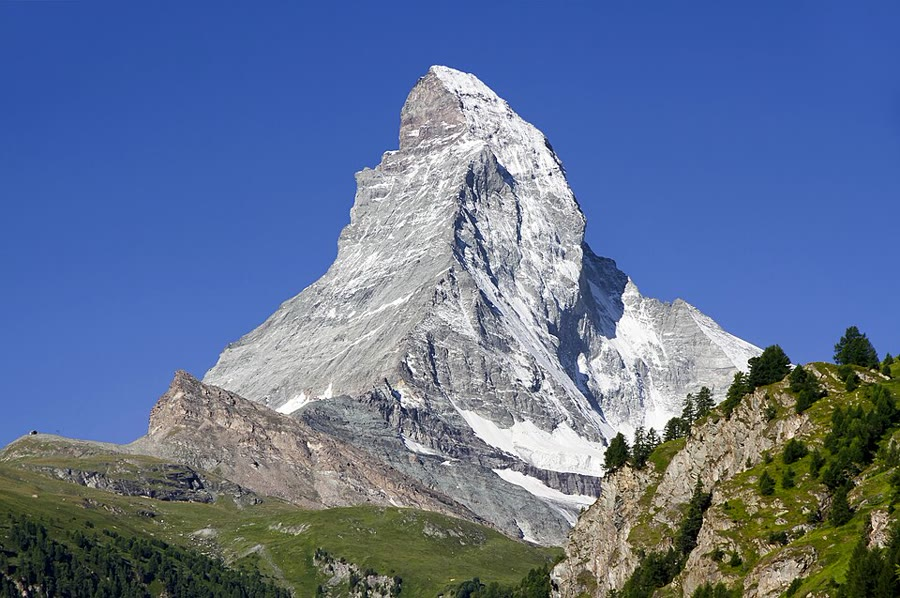
\includegraphics[width=0.7\linewidth]{images/book4/b2-13-matterhorn.jpg}
\par\smallskip{\small The north-east side of the Matterhorn (\qty{4478}{m}), seen from Zermatt:
its upper pyramid is Apulian gneiss and gabbro of the Dent Blanche thrust system, a \omterm{def:b2:alpine-orogen:klippe}{klippe}
on the \omterm{def:b2:alpine-orogen:ophiolite}{ophiolites} of the Alpine Tethys. Photograph Ximonic (Simo Räsänen), CC BY-SA
4.0.}
\end{omfigure}
% ledger: ispra16:cervino

\subsection*{Detachments and the two skins}

\omterm{def:b2:alpine-orogen:nappes}{Nappes} and thrust sheets move on surfaces of weakness.

\begin{definition}[Décollement]\label{def:b2:alpine-orogen:decollement}
A \emph{décollement}\index{decollement@décollement} is a low-angle surface along which a
sequence of rocks is detached from those beneath and slides over them, both sides deforming
independently; it usually follows a weak layer such as evaporite or shale.
\end{definition}

\begin{definition}[Thin-skinned and thick-skinned tectonics]\label{def:b2:alpine-orogen:skin}
\emph{Thin-skinned tectonics}\index{thin-skinned tectonics} is deformation of a
sedimentary cover detached from its basement along a basal \omterm{def:b2:alpine-orogen:decollement}{décollement}: the cover folds and
thrusts while the basement beneath stays undeformed. \emph{Thick-skinned
tectonics}\index{thick-skinned tectonics} is deformation in which the basement is involved,
cover and basement shortening together on faults that cut down into the basement.
\end{definition}
% ledger: lanza22:jura

\begin{definition}[Fold--thrust belt]\label{def:b2:alpine-orogen:ftb}
A \emph{fold--thrust belt}\index{fold--thrust belt} is a belt of folds and thrust faults
that shortens the outer part of an \omterm{def:b2:alpine-orogen:orogen}{orogen} and propagates towards its foreland; thrusts
step up from the \omterm{def:b2:alpine-orogen:decollement}{décollement} through the layers, and folds grow above them.
\end{definition}

The Alps have both skins. The Helvetic \omterm{def:b2:alpine-orogen:nappes}{nappes} are a thin-skinned \omterm{def:b2:alpine-orogen:ftb}{fold--thrust belt}, the
Mesozoic limestones of the near European margin detached from their basement. Their base is
the Glarus thrust, where Permian red beds lie on Cenozoic \omterm{def:b2:alpine-orogen:foreland}{flysch}. In the Miocene, by
contrast, basement blocks of the external massifs, shortened and thickened European basement (the
Aar, Mont Blanc, Belledonne, Pelvoux and Argentera massifs), were thrust up with their
cover: thick-skinned thrusting.
% ledger: schmid04:units, schmid04:skins, herwegh08:glarus, rosenberg21:massifs

The Jura, the arc of ridges north-west of the Swiss plain, is the classic example of thin
skin. In the late Miocene and Pliocene its Mesozoic cover was folded and thrust above a
\omterm{def:b2:alpine-orogen:decollement}{décollement} in the weak Middle and Upper Triassic evaporites, while the basement beneath
it, which continues from the external massifs under the \omterm{def:b2:alpine-orogen:foreland}{Molasse} basin, was not involved: on
the classic reading, the push came from the distant external massifs. Seismology has since
added a thick-skinned chapter. The earthquakes at Saint-Ursanne in 2000 had their source
less than a kilometre down and a thrust mechanism, active shallow thrusting in the cover,
while other studies find basement faults reactivated since the latest Pliocene. Whether
the Jura is still detached from its basement is debated.
% ledger: lanza22:jura, schmid04:skins

\begin{inthefield}[Reading a thrust contact]
Between Flims and the Walensee in eastern Switzerland runs the Glarus thrust, one of the
most prominent large low-angle thrusts of the Alps. Along it, Permian red beds, the
Verrucano, lie above Cenozoic \omterm{def:b2:alpine-orogen:foreland}{flysch}, far older rocks resting on younger ones. Between them, a
thin, strongly sheared band of limestone forms the contact: the Lochseiten limestone, on which the displacement, at least 30 to
\qty{40}{km}, was concentrated. In the nineteenth century Heim read the structure as two huge
overturned folds facing each other; Escher von der Linth had read one overthrust, and the thrust reading prevailed. A geologist who meets such a contact checks
three things: whether older rocks lie on younger ones, which no ordinary bedding can do;
whether the layers on either side are cut off at the contact; and whether the contact
itself is a band of sheared, recrystallised rock rather than a bedding plane.
\end{inthefield}
% ledger: herwegh08:glarus

\section{Foreland basins: flysch and molasse}\label{sec:b2:alpine-orogen:foreland}

A mountain belt loads the plate it rides on, and the plate bends down in front of it.

\begin{definition}[Foreland basin; flysch; molasse]\label{def:b2:alpine-orogen:foreland}
A \emph{foreland basin}\index{foreland basin} is an elongate sedimentary basin that forms
between an \omterm{def:b2:alpine-orogen:orogen}{orogen} and the stable continent in front of it, where the plate is bent down by
the load of the thrust wedge; it is deepest next to the thrust front and is itself
progressively overthrust. \emph{Flysch}\index{flysch} is the deep-water fill of such a
basin, chiefly turbidites of sandstone and shale deposited while the basin is underfilled.
\emph{Molasse}\index{molasse} is its later shallow-marine and continental fill, chiefly
conglomerates and sandstones from the eroding belt, deposited once the supply fills the
basin.
\end{definition}
% ledger: sinclair97:trinity, schmid04:foreland, krenmayr99:molasse

The bending is elastic flexure of the lithosphere, treated in a Year 3
chapter; here only its effect on the basin matters. Sinclair described the early Alpine \omterm{def:b2:alpine-orogen:foreland}{foreland basin}, of Paleocene to Oligocene age,
as an ``underfilled trinity'': limestones on the continental side, hemipelagic mud in the
middle, deep-water turbidites against the thrust front. As the thrusts advanced, the basin
moved with them: across Switzerland its continental shoreline crept north-westwards at 8.5
to \qty{12.9}{mm} a year, and the basin migrated with an almost steady shape for at least
\qty{210}{km} over the European plate.
% ledger: sinclair97:trinity

The north Alpine \omterm{def:b2:alpine-orogen:foreland}{Molasse} basin, which stretches from the Maritime Alps to Vienna, began to
subside in the late Eocene. Lower Oligocene \omterm{def:b2:alpine-orogen:foreland}{flysch}, now found on top of the Helvetic
\omterm{def:b2:alpine-orogen:nappes}{nappes}, records a last deep-water stage; from the late Oligocene to the late Miocene, rivers
spread continental gravels and sands from the young mountains. The name is old: H.-B. de Saussure
introduced \emph{\omterm{def:b2:alpine-orogen:foreland}{molasse}} in 1779. The fill thickens towards the belt: in the
Austrian sector, to more than \qty{4000}{m} at the thrust front, and elsewhere in the basin
a single late Oligocene suite of river conglomerates is some \qty{4}{km} thick. The southern part of
the basin has been overridden: the Austrian outcrop belt, about \qty{60}{km} wide, is less
than a quarter of the basin's former width. The overridden \omterm{def:b2:alpine-orogen:foreland}{molasse} itself is caught in
the thrusts as the Subalpine \omterm{def:b2:alpine-orogen:foreland}{Molasse}, south-dipping slices of conglomerate along the
northern rim of the belt.
% ledger: schmid04:foreland, krenmayr99:molasse, gs18:conglomerates

South of the Alps, the Po plain lies on the little-deformed Adriatic foreland of the
Southern Alps. Its youngest, Pliocene and Pleistocene, sediments partly cover Alpine
structures unconformably and are partly deformed by the last thrusts of the Southern Alps
and of the Apennines.
% ledger: schmid04:foreland

\begin{omfigure}
\centering
\begin{tikzpicture}[x=0.5cm, y=0.6cm, font=\scriptsize]
\begin{scope}
\node[anchor=west, font=\scriptsize\bfseries] at (0,2.4) {(a) underfilled: flysch};
\fill[blue!8] (0,0) -- (12,0) -- (12,1.4) -- (9.0,1.4) -- (4,0.05) -- (0,0.05) -- cycle;
\fill[gray!25] (0,0) -- (12,-1.1) -- (12,-1.9) -- (0,-0.8) -- cycle;
\fill[omThm!30] (9.0,1.4) -- (12,2.2) -- (12,-1.1) -- (9.5,-0.87) -- cycle;
\fill[green!25!gray!40] (5.5,-0.5) -- (9.5,-0.87) -- (9.3,-0.35) -- (7.0,-0.2) -- cycle;
\node at (10.9,0.6) {wedge};
\node at (2,-0.45) {craton};
\node[anchor=north] at (7.3,-0.9) {turbidites};
\draw[->] (7.3,-0.95) -- (7.6,-0.55);
\end{scope}
\begin{scope}[xshift=6.4cm]
\node[anchor=west, font=\scriptsize\bfseries] at (0,2.4) {(b) overfilled: molasse};
\fill[gray!25] (0,0) -- (12,-1.1) -- (12,-1.9) -- (0,-0.8) -- cycle;
\fill[omThm!30] (8.5,1.6) -- (12,2.4) -- (12,-1.1) -- (9.0,-0.82) -- cycle;
\fill[yellow!40] (1.5,-0.13) -- (9.0,-0.82) -- (8.5,1.0) -- (5,0.35) -- cycle;
\fill[blue!8] (0,0) -- (1.5,-0.13) -- (5,0.35) -- (4,0.4) -- (0,0.4) -- cycle;
\node at (10.6,0.6) {wedge};
\node at (2,-0.45) {craton};
\node at (6.2,-0.05) {gravels, sands};
\end{scope}
\end{tikzpicture}
\par\smallskip{\small A \omterm{def:b2:alpine-orogen:foreland}{foreland basin} in two stages (schematic). (a)~Early on, the bent
plate subsides faster than sediment arrives: deep water against the thrust wedge, where
turbidites (\omterm{def:b2:alpine-orogen:foreland}{flysch}) accumulate. (b)~Later the eroding belt supplies more than the basin can
hold: rivers fill it with gravels and sands (\omterm{def:b2:alpine-orogen:foreland}{molasse}), and the wedge thrusts over its own
debris.}
\end{omfigure}
% ledger: sinclair97:trinity, schmid04:foreland

\section{Reading the history: sections and geophysics}\label{sec:b2:alpine-orogen:sections}

A map shows where the units are; a cross-section shows how they lie beneath, and it can be
tested.

\begin{definition}[Balanced cross-section]\label{def:b2:alpine-orogen:balanced}
A \emph{balanced cross-section}\index{balanced cross-section} is a cross-section of deformed
rocks, drawn parallel to the direction of transport, that can be restored to a geologically
reasonable undeformed state without gaining or losing rock: the lengths of marker beds and
the areas of rock units in the section are conserved between the deformed and the restored
states.
\end{definition}

The restoration is anchored by \emph{pin lines}, lines across the layers at the ends of the
section, chosen where the rocks did not slip past one another.

\begin{proposition}[Line-length and area balance]\label{prop:b2:alpine-orogen:balance}
Between two pin lines a distance $l$ apart in the deformed state, let a marker bed have a
length $l_0$ measured along the bed, and let a layer of original thickness $t$ have a
cross-sectional area $A$. If length and area are conserved in the plane of the section,
\begin{enumerate}
\item the bed was $l_0$ long before deformation, the shortening is
$e = 1 - l/l_0$ and the shortening distance is $S = l_0 - l$;
\item the restored length of the layer is $l_0 = A/t$;
\item if a marker horizon lay at a depth $d$ above a flat \omterm{def:b2:alpine-orogen:decollement}{décollement}, the area of rock
raised above the marker's original level, its \emph{excess area} $A_e$, equals $S\,d$;
hence $d = A_e/S$.
\end{enumerate}
\end{proposition}

\begin{omfigure}
\centering
% book's own geometry (figdata/bachelor-2/alps.py)
\begin{tikzpicture}
\begin{axis}[width=0.86\linewidth, height=4.0cm, axis equal image, xmin=-1.5, xmax=31.5,
  ymin=-7.5, ymax=4.8, axis lines=none, clip=false]
\addplot[omThm, line width=1.2pt] table[x=x_km, y=y_km] {figdata/out/bachelor-2-alps-chevron.dat};
\addplot[gray, line width=1.2pt] table[x=x_km, y=y_km] {figdata/out/bachelor-2-alps-chevron0.dat};
\draw[dashed] (axis cs:0,-7) -- (axis cs:0,4.3);
\draw[dashed] (axis cs:22.98,-1.2) -- (axis cs:22.98,4.3);
\draw[dashed] (axis cs:30,-7) -- (axis cs:30,-4.8);
\draw[<->] (axis cs:0,-1.4) -- node[below, font=\scriptsize] {$l = \qty{23.0}{km}$} (axis cs:22.98,-1.4);
\node[font=\scriptsize, anchor=south] at (axis cs:15,-5.9) {restored: $l_0 = \qty{30.0}{km}$};
\node[font=\scriptsize, anchor=west] at (axis cs:23.3,2.2) {limb dip \qty{40}{\degree}};
\node[font=\scriptsize, anchor=south] at (axis cs:0,4.3) {pin};
\node[font=\scriptsize, anchor=south] at (axis cs:22.98,4.3) {pin};
\end{axis}
\end{tikzpicture}
\par\smallskip{\small Line-length balance of a marker bed folded into chevrons with limbs
dipping \qty{40}{\degree} (above), and the same bed restored between its pin lines
(below), at true scale. Each limb keeps its length; the folded bed spans
$l = 30.0\cos\qty{40}{\degree} = \qty{23.0}{km}$, a shortening of $1 - \cos\qty{40}{\degree} =
\qty{23.4}{\percent}$.}
\end{omfigure}

\begin{proof}
(1) A bed that neither stretches nor shortens along its length keeps it; the shortening is
the fraction of length lost, as at school. (2) Before deformation the layer is a strip of
length $l_0$ and thickness $t$, of area $l_0 t$, and the area is conserved. (3) Before
deformation, the rock between the marker's level and the \omterm{def:b2:alpine-orogen:decollement}{décollement} filled a strip $l_0$
long and $d$ thick. After it, between the pin lines, the same rock fills a strip $l$ long
from the \omterm{def:b2:alpine-orogen:decollement}{décollement} up to the marker's original level, of area $l\,d$, plus the excess
area pushed above that level. Conservation gives $l_0 d = l\,d + A_e$, so $A_e = (l_0 -
l)\,d = S\,d$. The relation gives the depth of a hidden \omterm{def:b2:alpine-orogen:decollement}{décollement} from a measured excess
area and shortening.
\end{proof}


\begin{method}[Restoring a section]\label{met:b2:alpine-orogen:restore}
\begin{enumerate}
\item Choose a section parallel to the transport direction and two pin lines where there
was no slip between layers.
\item Measure each marker bed along its length between the pins, counting every part
repeated by a thrust.
\item Lay the beds out flat at their measured lengths, keeping the order of the layers,
and redraw the faults on the restored section: their cut-offs must line up, without gaps
or overlaps.
\item Compare: beds of the same thrust sheet must restore to the same length; the areas of
the layers, divided by their thicknesses, must give the same lengths too. A section that
fails is not admissible as drawn.
\end{enumerate}
\end{method}

Balancing is a test of a section, not a proof of it, and its assumptions matter. In the Jura
near the Chasseral, line-length balancing of the top of the Jurassic gives \qty{5.1}{km} of
displacement, but area balancing and forward modelling give \qty{11.3}{km}: the extra
\qty{6.2}{km} was carried along a second, upper detachment in the Jurassic shales and passed
on to folds further north. One marker bed had missed half of the movement. The same study
weighed, and did not need, two other readings common in the Jura: basement highs pushing
up the folds, and anticline cores thickened by Triassic evaporites flowing into them, a
process that defeats area balance, since the evaporite layer no longer keeps its
thickness.
% ledger: schori15:chasseral, schori15:evaporite-flow

\subsection*{How much shortening?}

Applied to whole transects, balancing gives the bulk shortening of the belt, and the answers
differ with the assumptions. Across the Central Alps, along the NFP-20 transect, estimates
of collisional shortening have been about \qty{125}{km} in earlier work, \qty{160}{km} in
a 2015 compilation and \qty{144}{km} in a 2021 review; adding the dextral slip on the Periadriatic Line, which
moved Apulia sideways along the belt, raises the bulk convergence to between 206 and
\qty{250}{km}, depending on how much slip is assumed. In the Western Alps the estimates
range from 124 to \qty{243}{km}. Every one of them is a sum of restored pieces, each with
its own pin lines and its own guesses about what erosion and subduction removed.
% ledger: rosenberg21:shortening

\subsection*{What the geophysics sees}

Sections at depth rest on geophysics. Deep seismic reflection profiles have been shot
across the belt (ECORS--CROP in the Western Alps, NFP-20 West and East in
Switzerland, TRANSALP in the east), and dense networks of seismometers now map the Moho
from receiver functions, the conversions of teleseismic P waves into S waves at the base of
the crust. The AlpArray map, built from more than a hundred thousand receiver functions,
finds the Moho at about \qty{30}{km}, typical of continents, around the belt, and at 55 to
\qty{60}{km} beneath the Alps; the European Moho dips gently from about \qty{30}{km} in the
north-west to about \qty{55}{km} under the range.
The schematic section below sums up how the NFP-20 profiles across the Central Alps are
read.
% ledger: schmid04:transects, michailos23:moho

\begin{omfigure}
\centering
\begin{tikzpicture}[x=0.6cm, y=0.5cm, font=\scriptsize]
% surface and cover
\fill[yellow!30] (0,0) -- (3.0,0) -- (6.5,-0.3) -- (8.0,0.4) -- (8.0,-0.9) -- (0,-0.6) -- cycle;
\fill[gray!12] (0,-0.6) -- (8.0,-0.9) -- (12.5,-4.5) -- (15,-3.5) -- (16.5,-6.6) -- (16,-8.3)
  -- (0,-5.0) -- cycle;
\fill[gray!35] (0,-5.0) -- (16,-8.3) -- (17.5,-10.0) -- (0,-6.0) -- cycle;
% Helvetic and Aar
\fill[cyan!25] (8.0,0.4) -- (10.0,1.6) -- (11.0,1.2) -- (9.5,-0.4) -- (8.0,-0.9) -- cycle;
\fill[gray!12] (8.0,-0.9) -- (9.5,-0.4) -- (11.0,1.2) -- (12.0,2.0) -- (12.8,0.2) -- (11.5,-1.8)
  -- (12.5,-4.5) -- cycle;
% Penninic stack
\fill[omThm!35] (12.0,2.0) -- (14.5,2.6) -- (17.0,2.2) -- (17.3,-1.0) -- (15.0,-3.5) -- (12.5,-4.5)
  -- (11.5,-1.8) -- (12.8,0.2) -- cycle;
% Austroalpine/Apulia and Southern Alps
\fill[orange!30] (17.0,2.2) -- (19.0,1.6) -- (24,0.2) -- (26,0) -- (26,-3.5) -- (20.5,-4.0)
  -- (17.3,-1.0) -- cycle;
\fill[brown!35] (17.3,-1.0) -- (20.5,-4.0) -- (19.0,-7.0) -- (16.5,-6.6) -- (15,-3.5) -- cycle;
\fill[gray!35] (20.5,-4.0) -- (26,-3.5) -- (26,-6.0) -- (19.0,-7.0) -- cycle;
\fill[yellow!30] (23.5,0.3) -- (26,0) -- (26,-0.5) -- (24.5,-0.3) -- cycle;
\draw[thick] (17.3,-1.0) -- (17.0,2.2);
\draw[thick] (8.0,-0.9) -- (12.5,-4.5);
\draw[dashed] (0,-6.0) -- (17.5,-10.0);
\draw[dashed] (19.0,-7.0) -- (26,-6.0);
\node at (2.2,-0.25) {Jura};
\node at (5.2,-0.35) {molasse};
\node at (9.0,0.15) {Helvetic};
\node at (10.6,-0.6) {Aar};
\node at (14.6,0.4) {Penninic nappes};
\node at (21.2,-0.9) {Southern Alps};
\node at (24.9,-0.3) {Po};
\node at (18.0,-4.8) {Ivrea};
\node[align=center] at (5,-3.0) {European crust};
\node[anchor=north] at (3.2,-7.4) {European Moho};
\node at (10,-9.3) {mantle};
\node at (23,-7.7) {mantle};
\node[anchor=north] at (23,-6.55) {Adriatic Moho};
\node[anchor=south, align=center] at (17.2,2.25) {Periadriatic\\Line};
\draw[-{Latex[length=2mm]}] (1.0,0.5) -- (0.0,0.5);
\node[anchor=south] at (0.5,0.5) {NW};
\draw[-{Latex[length=2mm]}] (25.0,1.2) -- (26.0,1.2);
\node[anchor=south] at (25.5,1.2) {SE};
\end{tikzpicture}
\par\smallskip{\small A schematic crustal section across the Central Alps, from the Jura to
the Po plain (not to scale; after the interpretations of the NFP-20 transects compiled by
Schmid and colleagues). The European crust, with the Jura folded off its top, dips beneath
the Helvetic \omterm{def:b2:alpine-orogen:nappes}{nappes}, the Aar massif and the Penninic \omterm{def:b2:alpine-orogen:nappes}{nappe stack}; south of the Periadriatic
Line, Apulian crust with the wedge of the Ivrea body sits above the European Moho, and the
Southern Alps are thrust southwards over the Po plain.}
\end{omfigure}
% ledger: schmid04:transects, schmid04:units, schmid04:apulia, schmid04:skins


\begin{omfigure}
\centering
% ledger: data:b4-etopo-alps, data:b4-alps-moho, michailos23:moho
\begin{tikzpicture}
\begin{groupplot}[group style={group size=1 by 2, vertical sep=0.25cm, x descriptions at=edge bottom},
  width=0.92\linewidth, xmin=0, xmax=300, tick label style={font=\scriptsize},
  label style={font=\small}]
\nextgroupplot[height=3.6cm, ymin=0, ymax=4000, ylabel={elevation (\unit{m})},
  ytick={0,1000,2000,3000,4000}, y tick label style={/pgf/number format/1000 sep={}},
  legend style={font=\scriptsize, at={(0.99,0.97)}, anchor=north east, draw=none, fill=none}]
\addplot[gray, line width=0.4pt] table[x=km, y=max_m] {figdata/out/bachelor-2-alps-swath.dat};
\addplot[omThm, line width=1pt] table[x=km, y=mean_m] {figdata/out/bachelor-2-alps-swath.dat};
\legend{swath maximum, swath mean}
\node[font=\scriptsize, anchor=south west] at (axis cs:2,2650) {A (Po plain)};
\node[font=\scriptsize, anchor=south east] at (axis cs:298,1500) {B};
\nextgroupplot[height=4.6cm, ymin=0, ymax=70, y dir=reverse, xlabel={distance north of
  \qty{45.3}{\degree} N along \qty{8}{\degree} E (\unit{km})}, ylabel={depth (\unit{km})},
  legend style={font=\scriptsize, at={(0.99,0.03)}, anchor=south east, draw=none, fill=none}]
\addplot[only marks, mark=*, mark size=1.6pt, black] table[x=km, y=moho_km] {figdata/out/bachelor-2-alps-moho.dat};
\addplot[omThm, dashed, line width=0.8pt] table[x=km, y=airy_km] {figdata/out/bachelor-2-alps-airy.dat};
\addplot[gray, densely dotted] coordinates {(0,30) (300,30)};
\legend{Moho picks, Airy prediction, \qty{30}{km}}
\end{groupplot}
\end{tikzpicture}
\par\smallskip{\small Profile A--B along \qty{8}{\degree} E. Top: mean and maximum
elevation of the ETOPO1 nodes in a swath \qty{0.25}{\degree} either side of the meridian.
Bottom: the Moho depths picked on this meridian in the AlpArray receiver-function map
(Michailos and colleagues, CC BY 4.0), and the Moho that local Airy isostasy would put under
the swath-mean relief, for a \qty{30}{km} crust and densities 2700 and
\qty{3300}{kg.m^{-3}}.}
\end{omfigure}

The profile above confronts the root with Airy's model of the Year 1
volume. Under the highest part of the profile, where the swath-mean relief reaches
\qty{2.74}{km} at \qty{46.5}{\degree} N, a local Airy root would put the Moho at
$30 + 4.5 \times 2.74 = \qty{42.3}{km}$; it is observed at \qty{36.3}{km}. About a hundred
kilometres further south, at the edge of the Po plain, where the mean relief is only
\qty{0.65}{km}, the observed Moho is the deepest of the profile, \qty{61.2}{km}. The root is not under the peaks: it is
displaced towards Apulia. Over the stretch where picks exist, its cross-section, measured
below \qty{30}{km}, is about \qty{2300}{km^2}, against about \qty{1500}{km^2} for the Airy
roots of the relief above it. Local compensation of the present topography does not
explain the root. Pfiffner and colleagues point to an extra load: the Ivrea body, a wedge of
Adriatic mantle and lower crust within the belt, which helped bend the European plate
down.
% ledger: data:b4-etopo-alps, data:b4-alps-moho, michailos23:moho, pfiffner02:ivrea

Gravity tells the same story in another way. The pan-Alpine Bouguer anomaly map shows an
Alpine gravity low of $-100$ to \qty{-170}{mGal} along the range, deepest in the Central
Alps, from the light crust of the thickened root; a Po basin low of about $-80$ to
\qty{-140}{mGal}; and, between the Western Alps and the Po plain, the narrow Ivrea gravity
high, up to \qty{+40}{mGal}, where that dense lower crust and mantle come close to the
surface.
% ledger: zahorec21:gravity

\section{A timeline of the Alps}\label{sec:b2:alpine-orogen:timeline}

Gathering the dates of this chapter gives the belt's history in one table
(table below).

\begin{omfigure}
\centering\small
\begin{tabular}{p{0.28\linewidth}|p{0.62\linewidth}}
time & event \\ \hline
Middle Jurassic & the Piemont--Liguria ocean opens; its gabbros crystallise at
\qty{164}{Ma} \\
earliest Cretaceous & the Valais ocean opens north of the Briançonnais \\
about \qty{100}{Ma} & high-pressure peak of the Cretaceous orogeny in the eastern Alps \\
Late Cretaceous & the Apulian margin (Sesia zone) is subducted; the Apulian margin of the
ocean is active \\
48 to \qty{44}{Ma} & the Zermatt--Saas ocean floor reaches its deepest point, coesite and
diamond at Lago di Cignana \\
middle to late Eocene & the Valais ocean closes; the \omterm{def:b2:alpine-orogen:foreland}{Molasse} basin starts to subside \\
\qty{35}{Ma} & continental crust of the Dora Maira at ultrahigh pressure \\
Oligocene and Miocene & the Glarus thrust; \omterm{def:b2:alpine-orogen:foreland}{molasse} gravels fill the northern foreland (late
Oligocene to late Miocene) \\
Miocene & thick-skinned uplift of the external massifs; the Southern Alps thrust
southwards \\
late Miocene to Pliocene & thin-skinned folding of the Jura \\
today & levelling shows relative rock uplift of up to \qty{1.3}{mm} a year in the core of
the Central Alps
\end{tabular}
\par\smallskip{\small The Alps in eleven steps; the sources are cited in the sections
above.}
\end{omfigure}
% ledger: schmid04:alpine-tethys, rubatto98:zsf, schmid04:two-orogenies, halama20:cignana, schmid04:foreland, rh01:exhumation, herwegh08:glarus, schmid04:skins, schmid04:apulia, champagnac09:uplift

The last line is not the end of convergence. Repeated levelling across the Central Alps
gives relative rock uplift from about \qty{-0.4}{mm} a year north of the Jura to
\qty{1.3}{mm} a year in the core of the range, while GPS measurements suggest that the
Central Alps are not converging today. Champagnac and colleagues read the uplift as the isostatic rebound of a
crust being unloaded by erosion: the mountains rise because they are worn down.
% ledger: champagnac09:uplift

\section*{Exercises}\label{sec:b2:alpine-orogen:exercises}

Data for the exercises: $g = \qty{9.8}{m.s^{-2}}$,
$G = \qty{6.674e-11}{m^3.kg^{-1}.s^{-2}}$.

\begin{exercise}[$\star$]\label{exo:b2:alpine-orogen:1}
In a cross-section, a limestone bed measured along its folds between two pin lines is
\qty{36.0}{km} long; the pin lines are \qty{27.0}{km} apart. (a) Using
\cref{prop:b2:alpine-orogen:balance}, compute the shortening $e$ and the shortening distance
$S$. (b) What has to be true of the bed for the answer to hold?
\end{exercise}

\begin{exercise}[$\star$]\label{exo:b2:alpine-orogen:2}
On a geological map, (a) an oval patch of gneiss \qty{4}{km} long lies on Jurassic
limestone, its boundary a thrust that dips inwards, beneath the gneiss, all round; (b) an
elongate area of Cretaceous shale is surrounded by gneiss, along a thrust that dips
outwards, beneath the gneiss, all round. Name each structure and say what erosion has done
in each case.
\end{exercise}

\begin{exercise}[$\star$]\label{exo:b2:alpine-orogen:3}
(a) List the four units of the \omterm{def:b2:alpine-orogen:ophiolite}{Penrose ophiolite sequence} from bottom to top, and match each
with a layer of the oceanic crust or mantle. (b) The Chenaillet \omterm{def:b2:alpine-orogen:ophiolite}{ophiolite} shows exposed
mantle, gabbro and pillow basalts, and no sedimentary cover. Which Penrose unit does this
list leave out? (c) Why do \omterm{def:b2:alpine-orogen:ophiolite}{ophiolites} not give a fair sample of the floor of the wide
oceans?
\end{exercise}
% ledger: coleman84:penrose, coleman84:settings, corno23:chenaillet

\begin{exercise}[$\star$]\label{exo:b2:alpine-orogen:4}
On the way up the Matterhorn from the south, a climber crosses in turn the Monte Rosa and
Grand St Bernard \omterm{def:b2:alpine-orogen:nappes}{nappes}, the Zermatt--Saas \omterm{def:b2:alpine-orogen:ophiolite}{ophiolites}, the Combin zone and the gneisses of
the Dent Blanche thrust system. (a) Give the domain of origin of each. (b) Which plate was
the upper plate during subduction? (c) Why is this order a general rule in the \omterm{def:b2:alpine-orogen:nappes}{nappe stack},
and what can break it?
\end{exercise}
% ledger: ispra16:cervino, schmid04:units

\begin{exercise}[$\star\star$]\label{exo:b2:alpine-orogen:5}
The Central Alps carry a Bouguer anomaly of about \qty{-170}{mGal}. (a) Using the Bouguer
slab of the Year 1 volume, $\Delta g = 2\pi G\,\Delta\rho\,h$, find the thickness $h$ of an
infinite slab of density deficit $\Delta\rho = \qty{500}{kg.m^{-3}}$ (crust replacing mantle)
that gives this anomaly. (b) The receiver functions show a root of about \qty{25}{km} below a
\qty{30}{km} crust. What anomaly would an infinite slab that thick give? (c) Why is the
observed anomaly smaller?
\end{exercise}
% ledger: zahorec21:gravity, michailos23:moho

\begin{exercise}[$\star\star$]\label{exo:b2:alpine-orogen:6}
Gabbros of the Zermatt--Saas \omterm{def:b2:alpine-orogen:ophiolite}{ophiolite} crystallised at \qty{164}{Ma}; the \omterm{def:b2:alpine-orogen:ophiolite}{ophiolite} reached
its deepest point at \qty{44}{Ma}, at \qty{2.8}{GPa}. (a) How old was the oceanic
lithosphere when it was subducted? (b) Convert the pressure to depth with a mean overburden
density of \qty{3000}{kg.m^{-3}}, then \qty{3300}{kg.m^{-3}}. (c) Compare with the
``more than \qty{90}{km}'' quoted for this rock.
\end{exercise}
% ledger: rubatto98:zsf, halama20:cignana

\begin{exercise}[$\star\star$]\label{exo:b2:alpine-orogen:7}
A bed is folded into chevrons whose straight limbs all dip at the angle $\theta$.
(a) Show that the shortening is $e = 1 - \cos\theta$. (b) What limb dip gives
\qty{30}{\percent} shortening? (c) What shortening do limbs dipping \qty{40}{\degree} and
\qty{60}{\degree} give? Check the first against the chevron figure of the section on balancing.
\end{exercise}

\begin{exercise}[$\star\star$]\label{exo:b2:alpine-orogen:8}
A cover \qty{2.0}{km} thick is folded and thrust above a flat \omterm{def:b2:alpine-orogen:decollement}{décollement}. Between pin lines
now \qty{42}{km} apart, its cross-sectional area is \qty{118}{km^2}. (a) Find its restored
length, $S$ and $e$. (b) Compute the excess area and the depth of the \omterm{def:b2:alpine-orogen:decollement}{décollement} below the
original top of the cover. (c) Is the result consistent?
\end{exercise}

\begin{exercise}[$\star\star$]\label{exo:b2:alpine-orogen:9}
Along the \qty{8}{\degree} E profile of this chapter, the swath-mean elevation is
\qty{2.74}{km} at \qty{46.5}{\degree} N, where the Moho is picked at \qty{36.3}{km}, and
\qty{0.65}{km} at \qty{45.55}{\degree} N, where it is picked at \qty{61.2}{km}. (a) With a
\qty{30}{km} reference crust, $\rho_c = \qty{2700}{kg.m^{-3}}$ and $\rho_m =
\qty{3300}{kg.m^{-3}}$, compute the Airy Moho depth at both places. (b) Compare with the
picks. (c) What does the comparison say about how the Alpine root is held?
\end{exercise}
% ledger: data:b4-etopo-alps, data:b4-alps-moho, pfiffner02:ivrea

\begin{exercise}[$\star\star\star$]\label{exo:b2:alpine-orogen:10}
In the Chasseral section of the Jura, line-length balancing of the top of the Jurassic
gives \qty{5.1}{km} of displacement; area balancing and modelling give \qty{11.3}{km}, of
which \qty{6.2}{km} was carried along an upper detachment in Middle Jurassic shales.
(a) What fraction of the displacement did the top-Jurassic bed record? (b) Show that the
numbers add up, and explain why the upper bed misses part of the movement. (c) What
general lesson does this give for balancing with a single marker bed?
\end{exercise}
% ledger: schori15:chasseral

\begin{exercise}[$\star\star\star$]\label{exo:b2:alpine-orogen:11}
Across the Central Alps, about \qty{200}{km} of north-directed shortening has been
estimated, and the Periadriatic Line has an east--west dextral offset of about
\qty{100}{km}, perhaps 50, perhaps 150. (a) Add the two as perpendicular vectors and give
the bulk convergence for each offset. (b) What angle does the convergence make with the
north--south direction for an offset of \qty{100}{km}? (c) Why does the choice of offset
matter more than the third significant figure of the shortening?
\end{exercise}
% ledger: rosenberg21:shortening

\begin{exercise}[$\star\star\star$]\label{exo:b2:alpine-orogen:12}
The Swiss part of the Alpine \omterm{def:b2:alpine-orogen:foreland}{foreland basin} migrated at least \qty{210}{km} north-westwards
over Europe, its shoreline advancing at 8.5 to \qty{12.9}{mm} a year. (a) Over what range of
durations did the migration last? (b) In the Austrian sector, the present outcrop belt,
about \qty{60}{km} wide, is less than a quarter of the basin's former width. What was the
least former width, and how much of the basin is hidden under the thrusts? (c) Why can a
\omterm{def:b2:alpine-orogen:foreland}{foreland basin} never be fully preserved?
\end{exercise}
% ledger: sinclair97:trinity, krenmayr99:molasse

\begin{problem}[{Weekend problem --- restoring the section}]\label{pb:b2:alpine-orogen:1}
An Alpine-type \omterm{def:b2:alpine-orogen:orogen}{orogen} is crossed by a model section (an invented geometry, the book's own,
labelled as a model) made of five domains, from the foreland to the far side:
a foreland \omterm{def:b2:alpine-orogen:ftb}{fold--thrust belt}, \qty{48}{km} wide today; an external \omterm{def:b2:alpine-orogen:nappes}{nappe stack}, \qty{15}{km};
a basement massif, \qty{22}{km}; an internal zone of continental \omterm{def:b2:alpine-orogen:nappes}{nappes} and \omterm{def:b2:alpine-orogen:ophiolite}{ophiolites},
\qty{20}{km}; and a south-verging retro-wedge, \qty{48}{km}
(figure below). Lengths are in kilometres throughout.

\begin{omfigure}
\centering
\begin{tikzpicture}[x=0.075cm, y=0.5cm, font=\scriptsize]
\fill[yellow!30] (0,0) rectangle (48,1);
\fill[cyan!25] (48,0) rectangle (63,1);
\fill[gray!25] (63,0) rectangle (85,1);
\fill[omThm!35] (85,0) rectangle (105,1);
\fill[orange!30] (105,0) rectangle (153,1);
\draw (0,0) rectangle (153,1);
\foreach \x in {48,63,85,105} \draw (\x,0) -- (\x,1);
\node at (24,0.5) {foreland belt};
\node[align=center] at (55.5,1.6) {nappes};
\node at (74,0.5) {massif};
\node[align=center] at (95,1.6) {internal};
\node at (129,0.5) {retro-wedge};
\node[anchor=north] at (24,0) {48}; \node[anchor=north] at (55.5,0) {15};
\node[anchor=north] at (74,0) {22}; \node[anchor=north] at (95,0) {20};
\node[anchor=north] at (129,0) {48};
\end{tikzpicture}
\par\smallskip{\small The model section of the weekend problem: present widths of its
five domains, in kilometres (153 in all; an invented geometry).}
\end{omfigure}

\noindent\textbf{Part I --- Line-length balance of the foreland belt.} Between its two pin
lines, \qty{48.0}{km} apart, the top of the main limestone is made of ten straight segments
(horizontal extent $\Delta x$, dip), listed from the foreland; in addition, a thrust sheet
covers a flat stretch of the same bed, \qty{6.0}{km} long, which is repeated beneath it.

\smallskip
\begin{center}\small
\begin{tabular}{l|cccccccccc}
segment & 1 & 2 & 3 & 4 & 5 & 6 & 7 & 8 & 9 & 10\\ \hline
$\Delta x$ (\unit{km}) & 8.0 & 3.0 & 3.0 & 5.0 & 2.5 & 2.5 & 6.0 & 4.0 & 4.0 & 10.0\\
dip (\unit{\degree}) & 0 & 35 & 35 & 0 & 50 & 50 & 10 & 40 & 40 & 5
\end{tabular}
\end{center}
\smallskip

\begin{enumerate}
\item Compute the length along the bed of segments 2, 5 and 8.
\item Compute the total length of the bed between the pin lines, including the repeated
stretch.
\item Why must the stretch hidden under the thrust sheet be counted?
\item Compute the shortening $e$ and the shortening distance $S$ of the foreland belt.
\item The base of the limestone, measured the same way, is \qty{60.2}{km} long. By how much,
and by what percentage, do the two beds disagree? Is the section acceptable?
\item What would a length of \qty{54.0}{km} for the base have meant?
\end{enumerate}

\noindent\textbf{Part II --- Area balance and the décollement.} The cover between the
\omterm{def:b2:alpine-orogen:decollement}{décollement} and the top of the limestone was \qty{2.4}{km} thick before deformation; its
area between the pin lines is measured as \qty{146}{km^2}.
\begin{enumerate}[resume]
\item Compute the restored length of the cover from its area.
\item Compare with the line-length result of question~2.
\item Compute the excess area, raised above the cover's original top.
\item Deduce the depth of the \omterm{def:b2:alpine-orogen:decollement}{décollement} below that level, and compare it with the cover
thickness.
\item Had the area been \qty{160}{km^2}, what restored length would it give? Which process,
named in the Jura, could make the area and the line length disagree that way?
\item Why is this belt thin-skinned, and what should the top of the basement look like
beneath it?
\end{enumerate}

\noindent\textbf{Part III --- The external nappes and their pace.} The marker bed of the
three external \omterm{def:b2:alpine-orogen:nappes}{nappes} restores to 22, 18 and \qty{25}{km}; the stack now spans
\qty{15}{km}. In the basement massif, the top of the basement restores to \qty{30}{km}
against \qty{22}{km} today. The foreland belt deformed between 11 and \qty{4}{Ma}, the
\omterm{def:b2:alpine-orogen:nappes}{nappes} between 30 and \qty{20}{Ma}.
\begin{enumerate}[resume]
\item Compute the restored length of the \omterm{def:b2:alpine-orogen:nappes}{nappe stack} and its shortening distance.
\item Compute its shortening $e$ and compare it with that of the foreland belt.
\item Compute the shortening of the basement massif. What kind of tectonics is this?
\item Compute the mean shortening rates of the foreland belt and of the \omterm{def:b2:alpine-orogen:nappes}{nappes}, in
millimetres a year.
\item In which direction did deformation migrate through the section? Is this the order
of the Alps?
\item Add up the shortening of the three external domains.
\end{enumerate}

\noindent\textbf{Part IV --- The internal zone, the ocean and the whole section.}
\omterm{def:b2:alpine-orogen:ophiolite}{Ophiolite} slivers in the internal zone restore to \qty{18}{km}. Suppose that the ocean was
subducted from 85 to \qty{45}{Ma} at a mean rate of \qty{0.5}{cm} a year. The continental
\omterm{def:b2:alpine-orogen:nappes}{nappes} of the internal zone restore to \qty{60}{km} against \qty{20}{km} today, and the
marker bed of the retro-wedge to \qty{70}{km} against \qty{48}{km}.
\begin{enumerate}[resume]
\item What length of oceanic lithosphere was subducted?
\item Give a minimum width for the ocean.
\item Why is it only a minimum?
\item Compute the shortening of the internal zone and of the retro-wedge.
\item Add up the collisional shortening of the five domains, and compare it with the
estimates for the Central Alps in this chapter.
\item Crustal check: restore the section to its full width with a \qty{30}{km} crust, and
compare the crustal area with today's, a mean of \qty{45}{km} over the present
\qty{153}{km}. What fraction of the crust is missing from the present section, and where
did it go? Give the total collisional shortening across the section, rounded to the
kilometre.
\end{enumerate}
\end{problem}
